\chapter{FUNDAMENTAÇÃO TEÓRICA}
\label{FundamentacaoTeorica}

\section{Modelo de Banco de Dados Relacional}

O modelo Relacional surgiu por volta dos anos de 1970, com base no modelo proposto por Codd \cite{codd1970relational}. Através desse modelo, os dados são armazenados com um forte grau de independência, desacoplando a lógica, da representação dos dados \cite{davoudian2018survey}. Na representação Relacional, os dados são normalizados e as diversas relações (tabelas) podem referenciar os dados contidos em outras tabelas.

\hl{Cada linha de uma tabela (tupla) deve representar a abstração de um objeto do sistema}, sendo que \hl{cada célula da tupla é uma característica (atributo) do objeto representado}. Cada tupla \hl{deve possuir} pelo menos uma célula como identificador único (chave primária) que irá \hl{representar todos os dados contido na tupla} a qual ela está contida. A chave primária é um \hl{valor único} para a tabela, geralmente representado com um tipo numérico.

%%%%%
% Referenciar trabalhos científicos ou livros que apresentem as informações destacadas no parágrafo anterior
%%%%%

Caso seja necessário armazenar os dados contidos em uma tupla de outra relação, basta, em alguma célula da tupla, armazenar uma \hl{chave estrangeira} de outra tabela. Uma chave estrangeira é a chave primária de uma tupla de outra relação. Ao armazenar como chave estrangeira a chave primária de outra tabela, é realizado um link lógico, simbolizando que todos os dados representados por esta chave estrangeira também estão contidos dentro desta mesma tupla.

%%%%%
% Refereciar trabalhos científicos ou livros que apresentem as informações destracadas sobre chave estrangeira
%%%%%

Como exemplo, pode-se abstrair um sistema que precisa armazenar várias pessoas, na qual cada uma possui um nome e uma idade. \hl{Neste exemplo} pode-se representar os dados da seguinte forma:

\begin{table}[h]
    \centering
    \begin{tabular}{|c|c|c|}
        \hline
        \rowcolor[HTML]{FFAC71} 
        \multicolumn{3}{|c|}{\cellcolor[HTML]{FFAC71}Pessoa}                                                                                          \\ \hline
        \rowcolor[HTML]{9698ED} 
        {\color[HTML]{000000} \begin{tabular}[c]{@{}c@{}}Chave \\ Primária\end{tabular}} & {\color[HTML]{000000} Nome} & {\color[HTML]{000000} Idade} \\ \hline
        1                                                                                & Emanuel                     & 21                           \\ \hline
        2                                                                                & Eduardo                     & 40                           \\ \hline
    \end{tabular}
\end{table}

\hl{Nesse exemplo}, pode-se também desejar armazenar várias casas, na qual uma casa terá a sua rua e número. Neste caso é possível criar uma nova relação para a entidade (abstração de um tipo de objeto em nosso sistema) Casa:

\newpage

\begin{table}[h]
    \centering{
        \begin{tabular}{|c|c|c|}
            \hline
            \rowcolor[HTML]{67FD9A} 
            \multicolumn{3}{|c|}{\cellcolor[HTML]{67FD9A}Casa}                                                                                            \\ \hline
            \rowcolor[HTML]{9698ED} 
            {\color[HTML]{000000} \begin{tabular}[c]{@{}c@{}}Chave \\ Primária\end{tabular}} & {\color[HTML]{000000} Rua} & {\color[HTML]{000000} Número} \\ \hline
            10                                                                               & Rua Castelo Branco         & 1B                            \\ \hline
            20                                                                               & Rua Pompel                 & 1089                          \\ \hline
        \end{tabular}
    }
\end{table}

Continuando com o exemplo, naturalmente, no desenvolvimento de um sistema, as entidades se relacionam entre si. Neste caso, uma pessoa pode possuir várias casas, mas uma casa possui apenas uma pessoa como dono. Para representar essa relação, precisa-se definir quem será o dono da relação, ou seja, quem irá receber a chave primária da outra entidade através de uma chave estrangeira. Sempre deverá existir apenas  um dono da relação, ou seja, a chave estrangeira desta relação deverá estar em apenas uma tabela.
    
Como uma pessoa pode possuir várias casas, o dono da relação deve ser a casa, caso contrário a tupla de uma pessoa teria que ser duplicada (a menos que uma terceira tabela seja criada). Para representar essa situação pode-se modelar os dados da seguinte forma:
    
\begin{table}[h]
        \centering
        \begin{tabular}{|c|c|c|}
            \hline
            \rowcolor[HTML]{FFAC71} 
            \multicolumn{3}{|c|}{\cellcolor[HTML]{FFAC71}Pessoa}                                                                                          \\ \hline
            \rowcolor[HTML]{9698ED} 
            {\color[HTML]{000000} \begin{tabular}[c]{@{}c@{}}Chave \\ Primária\end{tabular}} & {\color[HTML]{000000} Nome} & {\color[HTML]{000000} Idade} \\ \hline
            1                                                                                & Emanuel                     & 21                           \\ \hline
            2                                                                                & Eduardo                     & 40                           \\ \hline
        \end{tabular}
    \end{table}
    
    \begin{table}[h]
        \centering
        \begin{tabular}{|c|c|c|c|}
            \hline
            \rowcolor[HTML]{67FD9A} 
            \multicolumn{4}{|c|}{\cellcolor[HTML]{67FD9A}Casa}                                                                                                                                                                        \\ \hline
            \rowcolor[HTML]{9698ED} 
            {\color[HTML]{000000} \begin{tabular}[c]{@{}c@{}}Chave \\ Primária\end{tabular}} & {\color[HTML]{000000} Rua} & {\color[HTML]{000000} Número} & \begin{tabular}[c]{@{}c@{}}Chave \\ Estrangeira \\ de Pessoa\end{tabular} \\ \hline
            10                                                                               & Rua Castelo Branco         & 1B                            & 1                                                                         \\ \hline
            20                                                                               & Rua Pompel                 & 1089                          & 1                                                                         \\ \hline
        \end{tabular}
\end{table}

Observando os dados exemplo apresentados acima, a pessoa Emanuel possui as duas casas armazenados no banco de dados, enquanto o Eduardo não possui nenhuma casa.

\subsection{Normalização}

O modelo Relacional possui algumas regras que o desenvolvedor \hl{deverá observar} ao modelar as estruturas das relações de seu banco. Dentre essas regras estão contidas as regras de normalização.

%%%%%
% As regras de nornalização realmente devem ser seguidas em todas circunstâncias?
%%%%%

A normalização é um conjunto de regras \hl{que visam, principalmente}, organizar os dados de forma a reduzir a redundância e otimizar a quantidade de dados armazenados.

%%%%%
% Justificar através de citações o parâgrafo anterior
%%%%%

Tal normalização pode ser dividida em seis formas normais. A seguir, serão explicadas as três primeiras formas normais, por serem as mais importantes e serem a de impacto mais significante para os propósitos deste trabalho.

\subsubsection{Primeira Forma Normal}
    
Como visto anteriormente, uma tupla representa um objeto da entidade representada pela relação a qual a tupla pertence. Tendo esse princípio como base, como é possível representar a situação de uma casa possuir vários donos e ao mesmo tempo uma pessoa possuir várias casas?
    
O princípio da primeira forma normal define que nunca deve-se duplicar tuplas, garantindo que duas ou mais tuplas nunca representem o mesmo objeto. Para manter este princípio e ainda realizar um relacionamento de muitos para muitos (uma pessoa tem muitas casas e uma casa tem muitas pessoas), torna-se necessário a criação de uma tabela auxiliar para representar o relacionamento de Pessoa com Casa:
    
\begin{table}[h]
        \centering
        \begin{tabular}{|c|c|c|}
            \hline
            \rowcolor[HTML]{FFAC71} 
            \multicolumn{3}{|c|}{\cellcolor[HTML]{FFAC71}Pessoa}                                                                                          \\ \hline
            \rowcolor[HTML]{9698ED} 
            {\color[HTML]{000000} \begin{tabular}[c]{@{}c@{}}Chave \\ Primária\end{tabular}} & {\color[HTML]{000000} Nome} & {\color[HTML]{000000} Idade} \\ \hline
            1                                                                                & Emanuel                     & 21                           \\ \hline
            2                                                                                & Eduardo                     & 40                           \\ \hline
        \end{tabular}
\end{table}
    
\begin{table}[h]
        \centering
        \begin{tabular}{|c|c|c|}
            \hline
            \rowcolor[HTML]{FCFF2F} 
            \multicolumn{3}{|c|}{\cellcolor[HTML]{FCFF2F}RelacionamentoPessoaCasa}                                                                                                                                                                                                                                   \\ \hline
            \rowcolor[HTML]{9698ED} 
            {\color[HTML]{000000} \begin{tabular}[c]{@{}c@{}}Chave \\ Primária do\\ Relacionamento\end{tabular}} & {\color[HTML]{000000} \begin{tabular}[c]{@{}c@{}}Chave \\ Estrangeira \\ de Pessoa\end{tabular}} & {\color[HTML]{000000} \begin{tabular}[c]{@{}c@{}}Chave \\ Estrangeira \\ de Casa\end{tabular}} \\ \hline
            100                                                                                                    & 1                                                                                                & 10                                                                                             \\ \hline
            200                                                                                                    & 1                                                                                                & 20                                                                                             \\ \hline
            300                                                                                                    & 2                                                                                                & 10                                                                                             \\ \hline
        \end{tabular}
\end{table}
    
\begin{table}[h]
        \centering
        \begin{tabular}{|c|c|c|}
            \hline
            \rowcolor[HTML]{67FD9A} 
            \multicolumn{3}{|c|}{\cellcolor[HTML]{67FD9A}Casa}                                                                                            \\ \hline
            \rowcolor[HTML]{9698ED} 
            {\color[HTML]{000000} \begin{tabular}[c]{@{}c@{}}Chave \\ Primária\end{tabular}} & {\color[HTML]{000000} Rua} & {\color[HTML]{000000} Número} \\ \hline
            10                                                                               & Rua Castelo Branco         & 1B                            \\ \hline
            20                                                                               & Rua Pompel                 & 1089                          \\ \hline
        \end{tabular}
\end{table}
    
No exemplo de modelagem acima, o Emanuel possui as duas casas e o Eduardo possui a casa de número 1B.
    
\subsubsection{Segunda Forma Normal}
    
A segunda forma normal especifica que todos os dados de uma tupla devem ser representados por toda a sua chave primária e jamais por apenas parte dela.
    
Como exemplo disso pode-se afirmar que uma casa jamais poderia ser armazenado dentro da mesma tupla de uma pessoa, mesmo em um relacionamento um para um (Uma Pessoa para uma Casa e uma Casa para uma Pessoa). Isto ocorre pois os dados de uma casa são independentes dos dados de uma pessoa e a chave primária de uma pessoa não poderia representar também os dados de uma casa.
    
Uma chave primária também pode ser composta por várias células, mas todos os dados da tupla devem depender de todas as células da chave primária e caso exista algum dado que dependa apenas de parte da chave primária, uma nova tabela deve ser criada. Uma tabela somente está na segunda forma normal se também estiver na primeira forma normal.
    
\subsubsection{Terceira Forma Normal}
    
Continuando o exemplo, pode-se imaginar que devem existir atributos no relacionamento entre pessoa e casa, indicando o valor mensal que a pessoa deve pagar como aluguel pela casa, a quantidade de meses a pagar o aluguel e o total a pagar até o fim do contrato. Para isso, poderíamos adicionar tais atributos na tabela de relacionamento de Pessoa Com Casa:
    
    \begin{table}[h]
        \centering
        \begin{tabular}{|c|c|c|c|c|c|}
            \hline
            \rowcolor[HTML]{FCFF2F} 
            \multicolumn{6}{|c|}{\cellcolor[HTML]{FCFF2F}RelacionamentoPessoaCasa}                                                                                                                                                                                                                                                                                                                                                                                                                      \\ \hline
            \rowcolor[HTML]{9698ED} 
            {\color[HTML]{000000} \begin{tabular}[c]{@{}c@{}}Chave \\ Primária do\\ Relacionamento\end{tabular}} & {\color[HTML]{000000} \begin{tabular}[c]{@{}c@{}}Chave \\ Estrangeira \\ de Pessoa\end{tabular}} & {\color[HTML]{000000} \begin{tabular}[c]{@{}c@{}}Chave \\ Estrangeira \\ de Casa\end{tabular}} & \begin{tabular}[c]{@{}c@{}}Valor\\ Mensal\end{tabular} & \begin{tabular}[c]{@{}c@{}}Quantidade\\ de Meses\end{tabular} & \begin{tabular}[c]{@{}c@{}}Total a\\ Pagar\end{tabular} \\ \hline
            100                                                                                                    & 1                                                                                                & 10                                                                                             & 200                                                    & 12                                                            & 2400                                                    \\ \hline
            200                                                                                                    & 1                                                                                                & 20                                                                                             & 400                                                    & 24                                                            & 9600                                                    \\ \hline
            300                                                                                                    & 2                                                                                                & 10                                                                                             & 300                                                    & 8                                                             & 2400                                                    \\ \hline
        \end{tabular}
    \end{table}
    
Neste exemplo, O Emanuel paga 200 reais pela Casa de número 1B com contrato válido por 12 meses e paga 400 reais pela casa de número 1089 com contrato válido por 24 meses. O Eduardo paga 300 reais pela casa de número 1B com contrato válido por 8 meses.
    
Para este caso, esta relação não está na terceira forma normal, pois o atributo \textit{Total a Pagar} é dependente do \textit{Valor Mensal} e da \textit{Quantidade de Meses}. O total a pagar pode ser obtido através de uma busca no banco de dados realizando uma simples multiplicação do \textit{Valor Mensal} e da \textit{Quantidade de Meses}. Para que esta relação fique de acordo com a Terceira Forma Normal é necessário remover a coluna \textit{Total a Pagar}:
    
\begin{table}[h]
    \centering
    \begin{tabular}{|c|c|c|c|c|}
        \hline
        \rowcolor[HTML]{FCFF2F} 
        \multicolumn{5}{|c|}{\cellcolor[HTML]{FCFF2F}RelacionamentoPessoaCasa}                                                                                                                                                                                                                                                                                                                                                            \\ \hline
        \rowcolor[HTML]{9698ED} 
        {\color[HTML]{000000} \begin{tabular}[c]{@{}c@{}}Chave \\ Primária do\\ Relacionamento\end{tabular}} & {\color[HTML]{000000} \begin{tabular}[c]{@{}c@{}}Chave \\ Estrangeira \\ de Pessoa\end{tabular}} & {\color[HTML]{000000} \begin{tabular}[c]{@{}c@{}}Chave \\ Estrangeira \\ de Casa\end{tabular}} & \begin{tabular}[c]{@{}c@{}}Valor\\ Mensal\end{tabular} & \begin{tabular}[c]{@{}c@{}}Quantidade\\ de Meses\end{tabular} \\ \hline
        1                                                                                                    & 1                                                                                                & 10                                                                                             & 200                                                    & 12                                                            \\ \hline
        2                                                                                                    & 1                                                                                                & 20                                                                                             & 400                                                    & 24                                                            \\ \hline
        3                                                                                                    & 2                                                                                                & 10                                                                                             & 300                                                    & 8                                                             \\ \hline
    \end{tabular}
\end{table}
    
A terceira forma normal especifica que não deve existir uma célula que dependa de outras células. Cada valor deverá ser o mais independente possível dos outros valores. Para que uma relação esteja na terceira forma normal, também torna-se necessário que esteja na segunda forma normal.

\subsection{Junção de Tabelas}
    
Existem situações onde as tabelas precisam ser unidas em uma única tabela desnormalizada, para a realização de buscas mais complexas, ou para simplesmente agrupar os dados da maneira como eles devem ser consumidos nas aplicações que os irão utilizar.
    
Como exemplo disto, pode-se unir as três tabelas exemplo apresentadas anteriormente, apenas para a pessoa de nome \textit{Emanuel}. A seguir encontra-se uma codificação SQL para a união de tabelas e logo em seguida a tabela resultante de tal codificação.

\begin{lstlisting}[language=SQL, caption={União de Tabelas com SQL}]
    SELECT * 
    FROM Pessoa p JOIN
        RelacionamentoPessoaCasa rpc ON p.id = rpc.pessoa_id JOIN
        Casa c ON rpc.casa_id = c.id
    WHERE p.nome = "Emanuel"
\end{lstlisting}
    
    \begin{table}[h]
        \centering
        \resizebox{\textwidth}{!}{%
            \begin{tabular}{|c|c|c|c|c|c|c|c|c|c|c|}
                \hline
                \rowcolor[HTML]{38FFF8} 
                \multicolumn{11}{|c|}{\cellcolor[HTML]{38FFF8}Junção das Três Tabelas}                                                                                                                                                                                                                                                                                                                                                                                                                                                                                                                                                        \\ \hline
                \rowcolor[HTML]{9698ED} 
                \begin{tabular}[c]{@{}c@{}}Chave\\ Primária\\ de Pessoa\end{tabular} & Nome    & Idade & {\color[HTML]{000000} \begin{tabular}[c]{@{}c@{}}Chave \\ Primária do\\ Relacionamento\end{tabular}} & {\color[HTML]{000000} \begin{tabular}[c]{@{}c@{}}Chave \\ Estrangeira \\ de Pessoa\end{tabular}} & {\color[HTML]{000000} \begin{tabular}[c]{@{}c@{}}Chave \\ Estrangeira \\ de Casa\end{tabular}} & \begin{tabular}[c]{@{}c@{}}Valor\\ Mensal\end{tabular} & \begin{tabular}[c]{@{}c@{}}Quantidade\\ de Meses\end{tabular} & \begin{tabular}[c]{@{}c@{}}Chave\\ Primária\\ de Casa\end{tabular} & Rua                & Número \\ \hline
                1                                                                    & Emanuel & 21    & 100                                                                                                    & 1                                                                                                & 10                                                                                             & 200                                                    & 12                                                            & 10                                                                 & Rua Castelo Branco & 1B     \\ \hline
                1                                                                    & Emanuel & 21    & 200                                                                                                    & 1                                                                                                & 20                                                                                             & 400                                                    & 24                                                             & 20                                                                 & Rua Pompel & 1089     \\ \hline
            \end{tabular}%
        }
    \end{table}
    
Neste caso, algumas colunas do relacionamento de Pessoa com Casa são desnecessárias e no comando de junção das tabelas pode-se omití-las. Neste caso a tabela de junção seria algo como:
    
    \begin{table}[h]
        \centering
        \resizebox{\textwidth}{!}{%
            \begin{tabular}{|c|c|c|c|c|c|c|c|}
                \hline
                \rowcolor[HTML]{38FFF8} 
                \multicolumn{8}{|c|}{\cellcolor[HTML]{38FFF8}Junção das Três Tabelas}                                                                                                                                                                                                                                              \\ \hline
                \rowcolor[HTML]{9698ED} 
                \begin{tabular}[c]{@{}c@{}}Chave\\ Primária\\ de Pessoa\end{tabular} & Nome    & Idade & \begin{tabular}[c]{@{}c@{}}Valor\\ Mensal\end{tabular} & \begin{tabular}[c]{@{}c@{}}Quantidade\\ de Meses\end{tabular} & \begin{tabular}[c]{@{}c@{}}Chave\\ Primária\\ de Casa\end{tabular} & Rua                & Número \\ \hline
                1                                                                    & Emanuel & 21    & 200                                                    & 12                                                            & 10                                                                 & Rua Castelo Branco & 1B     \\ \hline
                1                                                                    & Emanuel & 21    & 400                                                    & 24                                                             & 20                                                                 & Rua Pompel & 1089     \\ \hline
            \end{tabular}%
        }
    \end{table}

\hl{A ideia dos dados estarem separados é de tentar garantir} que os dados fiquem consistentes na hora de atualizar os dados existentes, além de tentar garantir uma velocidade maior na hora de atualizar valores, mas em buscas no banco de dados, as junções de tabelas são, muitas vezes, inevitáveis.

%%%%%
% Referenciar trabalhos que demonstrem que a separação dos dados tem o proposito apresentado no parágrafo anterior
%%%%%
    
Em um sistema complexo, com uma grande quantidade de dados e relações, cada tabela poderá conter milhares ou até milhões de linhas, envolvendo a junção de centenas de tabelas, podendo deixar essas operações de junção lentas demais para os requisitos da aplicação. \hl{Existem algumas técnicas e estratégias} para deixar essas consultas mais rápidas, mas mesmo com essas estratégias, haverá aplicações na qual a exigência de alta performance, escalabilidade, disponibilidade e consistência tornará inviável ou altamente caro escalar uma aplicação utilizando o modelo Relacional.

%%%%%
% Que técnicas são essas faladas no parágrafo anterior? Elas realmente existem? Buscar referencias binliográficas para fazer tal afirmação
%%%%%

\subsection{Vantagens do Modelo Relacional}

%%%%%
% Justificar tais vantagens por meio de referências bibliográficas
%%%%%
    
\begin{itemize}
    \item O modelo Relacional já está bem solidificado no mercado, possuindo várias
         ferramentas e frameworks para facilitar o desenvolvimento dos mais diversos tipos
         de aplicações;
        
    \item Pelo fato do modelo Relacional forçar a separação e normalização dos dados,
         torna-se mais difícil que erros humanos ou de desenvolvimento venham a fazer os
         dados perderem sua consistência;
        
%    \item A normalização dos dados proporciona que os dados possam ser
%         inseridos/atualizados sem que o usuário/desenvolvedor tenha a responsabilidade de 
%         fazer diversas verificações físicas/lógicas na própria estrutura de armazenamento de
%         dados;
        
%    \item Uma modelagem de dados mal planejada possui menos chances de causar grandes
%         danos a consistência dos dados por causa da normalização;
        
    \item A normalização, por causa de seu princípio de não repetir dados em várias tabelas,
         garante que os dados sejam armazenados utilizando pouco espaço de
         armazenamento;

    \item Por causa da normalização, a atualização de registros são, geralmente, bastante 
         rápidas.
\end{itemize}
    
\subsection{Desvantagens do Modelo Relacional}

%%%%%
% Justificar tais desvantagens por meio de referências bibliográficas
%%%%%
    
\begin{itemize}
    \item O modelo de dados relacionais possui recursos de modelagem muito limitados;
        
    \item O mapeamento de objetos com operação de junção, muitas vezes são caras;
        
    \item As demandas recentes de armazenamento e consulta de uma grande quantidade 
         de dados revelaram várias deficiências do relacionamento relacional tradicional;
        
    \item Diversos tipos de aplicações com altos requisitos de escalabilidade, disponibilidade e
          consistência podem se tornam caras ou inviáveis;
        
    \item As aplicações precisam se adaptar ao modelo Relacional. Mesmo que uma aplicação
         possa ter uma parte dos dados não normalizados sem prejudicar a consistência por
         causa de alguma regra de negócio, o modelo relacional exige a normalização para
         um bom funcionamento do SGBD.
\end{itemize}

\section{Modelo de Banco de Dados NoSQL com \textit{MongoDB}}
    
Desde o início dos anos 2000, os avanços na tecnologia web, resultaram na explosão repentina de dados estruturados, semi-estruturados e não estruturados por aplicativos de escopo global. Tais aplicações geralmente exigem uma escalabilidade horizontal, adaptar-se às enormes quantidades de dados e à taxa crescente de processamento de consultas \cite{davoudian2018survey}.
    
A alta disponibilidade, a baixa tolerância a falhas para responder aos clientes, confiabilidade de transações, o suporte a dados altamente consistentes e a manutenção de \textit{schemas} de banco de dados com baixo custo de evolução do sistema são requisitos que se tornam muitos difíceis ou inatingíveis nos sistemas tradicionais de banco de dados Relacional \cite{davoudian2018survey}.
    
Além desse motivo, a ampliação de sistemas exige uma movimentação de servidores autônomos com hardware aprimorados, sendo um processo caro e causa uma indisponibilidade significativa a cada movimentação. Sistemas baseados em modelos Relacionais exigem uma complexidade e sobrecarga maiores para se juntar dados distribuídos normalizados \cite{davoudian2018survey}.
    
\hl{De acordo com publicações recentes}, os requisitos acima podem ser resolvidos compensando ou sacrificando outros requisitos não tão necessários para a aplicação.

%%%%%
% Que publicações recentes?
%%%%%
    
Os modelos de banco de dados NoSQL tornaram-se uma tendência emergente de armazenamento de dados não relacional, que visam satisfazer os requisitos de alta disponibilidade e escalabilidade de aplicações de âmbito global \cite{davoudian2018survey}.
    
Um modelo de Banco de Dados NoSQL é caracterizado pela utilização de um modelo não relacional ou parcialmente relacional para o armazenamento de dados. Vários modelos NoSQL foram criados visando esses princípios acima descritos. Para os propósitos deste trabalho, esta seção utiliza como base a descrição e utilização de modelos de banco de dados Baseado em Documento, sendo exemplificado pela descrição e uso do banco de dados \textit{MongoDB}.

Enquanto que no modelo Relacional o armazenamento ocorre em uma tabela, no MongoDB o armazenamento ocorre em uma coleção de documentos, sendo cada documento a representação de um objeto do sistema. Cada banco de dados NoSQL baseado em Documento terá a sua própria estrutura de documento. No caso específico do \textit{MongoDB}, os documentos são escritos de maneira estruturada, seguindo uma variação do formato JSON (\textit{JavaScript Object Notation}). Tal variação possui o nome de BSON (\textit{Binary} JSON).

\subsection{O Formato JSON}
    
O JSON é um formato de representação de dados \hl{chave-valor}. A chave é o nome do atributo (caracterísica) pertencente ao objeto na qual o JSON representa. Uma chave é utilizada para representar o valor (valor da característica do objeto) a ela associada.

%%%%%
% A representação de dados feita pelo JSON pode realmente ser chamada de "chave-valor"? Essa pergunta é feita pois existe uma outra representação de dados que possui esse nome
%%%%%

O valor associado a uma chave pode ser do tipo textual (entre aspas), tipo numérico (sem aspas), pode ser um outro JSON (definido entre chaves) e pode ser uma lista de qualquer um dos tipos definidos anteriormente (entre colchetes separados por vírgula).
    
A seguir é apresentado um exemplo de representação de uma lista de pessoas com suas respectivas casas:

\newpage

\begin{lstlisting}[language=json, caption={JSON Representando Uma Lista de Pessoas Com Suas Casas}]
[{
    "nome": "Emanuel",
    "idade": 21,
    "casas": [
        {
            "rua": "Rua Castelo Branco",
            "numero": "1B",
            "valorMensal": 200,
            "quantidadeMeses": 12
        },
        {
            "rua": "Rua Pompel",
            "numero": 1089,
            "valorMensal": 400,
            "quantidadeMeses": 24
        }
    ]
},
{
    "nome": "Eduardo",
    "idade": 40,
    "casas": {
        "rua": "Rua Pompel",
        "numero": "1089",
        "valorMensal": 300,
        "quantidadeMeses": 8
    }
}]
\end{lstlisting}

Observa-se que a representação de um objeto é dada entre chaves (\textit{\{\}}) e, dentro dessas chaves, são definidos os nomes dos atributos do objeto e, após os dois pontos (\textit{:}), é definido o valor para aquele atributo. Quando se deseja que o valor seja uma lista de elementos, envolve-se todos os elemento da lista entre colchetes e cada elemento é separado por vírgula (\textit{,}).
    
No exemplo apresentado acima, está sendo representado uma lista de objetos. Para a representação desta lista, as pessoas (JSON) são envolvidas entre colchetes. Caso seja desejado representar apenas uma pessoa ao invés de uma lista, bastaria remover os colchetes mais externos e deixar apenas um JSON na raiz do documento. Observa-se que a pessoa com o nome \textit{Eduardo} possui apenas uma casa, e por este motivo o valor do atributo \textit{casa} pode ser representado como um JSON, mas também seria possível representar como uma lista de apenas uma casa, bastando para isso apenas envolver as chaves (\textit{\{\}}) em colchetes (\textit{[]}), assim como ocorre para a pessoa \textit{Emanuel}.

\subsection{Coleções de Documentos no MongoDB}
    
O formato de documento utilizado pelo MongoDB é uma variação do JSON: o BSON (\textit{Binary JSON}). O BSON é quase idêntico ao JSON, sendo qua a diferença \hl{é apenas} a adição de novos tipos, como um tipo para a representação de datas e um tipo para a representação de um identificador para o documento (o \textit{ObjectId}).

%%%%%
% Será que não existe outra diferença entre o JSON e o BSON não apresentada no parágrafo anterior?
%%%%%

Enquanto que no modelo Relacional uma tabela representa uma coleção de objetos no sistema, no \textit{MongoDB}, esta representação é feita por uma coleção de documentos. Da mesma forma, enquanto uma tupla de uma tabela representa, no modelo Relacional, um objeto, no \textit{MongoDB}, esta representação é feita por um documento. Cada documento possui, em seu interior, um BSON (não uma lista, mas apenas um único BSON).
    
Seguindo essa abordagem, para, por exemplo, armazenarmos várias pessoas em \hl{nosso} banco, precisa ser criado uma coleção que irá armazenar vários documentos, sendo cada documento uma representação BSON de uma pessoa diferente. Cada documento terá um identificador único para a coleção (\textit{\_id}) que irá  representar todo o documento. Através deste identificador, pode-se fazer relações entre documentos. Tal identificador pode ser de qualquer tipo, porém o tipo \hl{recomentado} é o \textit{ObjectId}. A seguir é listado algumas vantagens do uso do \textit{ObjectId}:

%%%%%
% Utilização de pronome em primeira pessoa no parágrafo anterior

% O uso do ObjectId é recomendado por quem? Existem situações onde esse tipo não é recomendado?
%%%%%

\begin{itemize}
    \item O \textit{ObjectId} é formado por 12 bytes, sendo os quatro primeiros refletidos no \textit{timestamp} de quando o documento foi criado e possui uma \hl{probabilidade muito alta} de ser único. Por causa disto, é possível obter a data de criação de um documento pelo identificador
    
    \item Odenar pelo \textit{\_id} com o tipo \textit{ObjectId} é equivalente a ordenar os documentos pela data de criação (para os documentos criados no mesmo segundo não é garantido nenhuma ordem)
    
    \item O campo \textit{\_id} é automaticamente criado caso não seja informado
\end{itemize}

%%%%%
% Qual a probabilidade do ObjectId ser único? Usar o termo "muito" pode ser inadequado
%%%%%

A seguir será exemplificado um BSON que poderia ser armazenado em um documento do \textit{MongoDB}. Para ilustrar a flexibilidade do valor do \textit{\_id}, o identificador das entidades serão armazenados por meio de um valor numérico, porém os identificadores dos BSON ``internos'' serão definidos como um \textit{ObjectId}. Esta escolha foi tomada apenas para facilitar a visualização dos exemplos, mas em um sistema, o \textit{\_id} poderia assumir qualquer tipo de dado.

\begin{lstlisting}[language=json, caption={Estrutura de Dados da Pessoa \textit{Emanuel}}]
{
    "_id": 1,
    "nome": "Emanuel",
    "idade": 21,
    "casas": [
        {
            _id: ObjectId("5e66c969d5d7cc24c0850854"),
            "rua": "Rua Castelo Branco",
            "numero": "1B",
            "valorMensal": 200,
            "quantidadeMeses": 12
        },
        {
            _id: ObjectId("5e66c9740efbf528b05a7537"),
            "rua": "Rua Pompel",
            "numero": 1089,
            "valorMensal": 400,
            "quantidadeMeses": 24
        }
    ]
}
\end{lstlisting}

O identificador (\textit{\_id}) deve existir pelo menos no BSON principal (neste caso, o BSON que representa uma pessoa). O BSON que representa uma casa não necessariamente precisa de um identificador, mas, para este exemplo, optou-se por gerar um. O identificador do BSON de uma casa não é o identificador de outro documento, pois neste exemplo os dados estão desnormalizados e, por enquanto, para o nosso exemplo, não existe outra coleção além da coleção de Pessoa.

\subsection{Desnormalização}

A desnormalização é o armazenamento de dados sem a preocupação de seguir as formas normais. No exemplo apresentado, a coleção de Casa não existe e as casas estão armazenadas dentro do mesmo BSON na qual uma pessoa é armazenada. Tal estrutura desobedece a terceira forma normal, pois o identificador do documento (\textit{\_id}) identifica uma pessoa, não podendo, portanto, identificar os dados das casas que estão presente no próprio documento.
    
Uma das principais vantagens da desnormalização é que não existe a necessidade de realizar junção de vários documentos, podendo ter um ganho substancial de performance. No exemplo apresentado do modelo Relacional, foi necessário realizar buscas e uniões de tabelas para obter uma tabela contendo um balanço da lista total de casas da pessoa com nome \textit{Emanuel}. No MongoDB, caso desejemos realizar a mesma pesquisa para a pessoa \textit{Emanuel}, obtendo a lista de casas que ela possui, não haveria a necessidade de juntar quaisquer documentos, bastando apenas buscar o documento da pessoa a qual se deseja buscar e retornar o documento tal qual como foi armazenado.
    
No modelo relacional, como foi abordado anteriormente, uma tabela pode ter milhares ou milhões de linhas e pode ser necessário unir centenas de tabelas. Com a desnormalização, nenhuma junção torna-se necessária para este caso.

\subsection{Limites da Desnormalização}
    
Apesar dos benefícios da desnormalização, ela nem sempre é aconselhável ou viável. Através da desnormalização, os dados começam a ser duplicados, e dependendo das regras da aplicação, essa duplicação pode ser problemática. Como exemplo disso, pode-se imaginar uma situação onde várias pessoas possuem uma mesma casa. Neste exemplo, os dados da mesma casa precisariam ser duplicados em diversas pessoas. Se uma casa nunca precisar ser removida ou atualizada, essa duplicação possivelmente não irá gerar nenhum problema, mas caso uma casa precise ser removida ou ter, por exemplo o seu número atualizado, seria necessário atualizar a casa em todas as pessoas que a possuem. Essa operação poderia ser extremamente lenta e dependendo da quantidade de dados armazenados, isto seria uma operação inviável. A desnormalização deve ocorrer em situações onde as regras de negócio da aplicação garantem uma segurança na realização de tal procedimento.
    
Quando a desnormalização completa não for uma opção, torna-se necessário a criação de uma nova coleção para normalizar esses dados. Para exemplificar esta normalização, uma nova coleção deve ser criada para armazenar todas as casas, e no atributo \textit{casas} no documento de pessoa, apenas será armazenado o identificador da casa a qual ela está relacionada, junto com os atributos de relacionamento \textit{valorMensal} e \textit{quantidadeMeses}.

A seguir é apresentado exemplos de como os dados seriam estruturados mediante uma normalização:
    
\begin{lstlisting}[language=json, caption={Estrutura de Dados Normalizados de uma Casa}]
{
    "_id": 20,
    "rua": "Rua Pompel",
    "numero": "1089"
}
\end{lstlisting}
    
\begin{lstlisting}[language=json, caption={Estrutura de Dados Normalizados da Pessoa \textit{Eduardo}}]
{
    "_id": 2,
    "nome": "Eduardo",
    "idade": 40,
    "casas": {
        "_id": ObjectId("5e66cad68a1e581e3cf47dfc"),
        "id": 20,
        "valorMensal": 300,
        "quantidadeMeses": 8
    }
}
\end{lstlisting}

Observa-se que no atributo de \textit{casas} existem dois identificadores. O identificador \textit{\_id} identifica o BSON do relacionamento de pessoa com casa. O identificador \textit{id} é um atributo que poderia ter recebido outro nome. Como neste caso é necessário armazenar o identificador do documento de casa, escolhe-se um nome de atributo que será padronizado na aplicação para referenciar a casa a qual esta pessoa se relaciona. Neste exemplo, escolheu-se padronizar o atributo \textit{id} como aquele que receberá o identificador do documento da casa que se relaciona com esta pessoa. Desta forma, o identificador da casa a qual esta pessoa pertence (20) será armazenado no atributo \textit{id}. 

É possível padronizar para que o \textit{\_id} represente, ao mesmo tempo, o identificador do BSON (identificador do relacionamento) e o identificador da entidade relacionada. Nesse caso, o atributo \textit{id} não seria necessário. Para as exemplificações desse trabalho, essa padronização não será feita, pois ter esses dois identificadores pode gerar algumas vantagens em consultas. Uma possível vantagem seria a de uma entidade poder se relacionar mais de uma vez com o mesmo documento, de mesmo identificador (\textit{id}), porém o sistema poderia diferenciar os dois relacionamentos por meio do identificador da relação (\textit{\_id}). Além dessa vantagem, pode ser que alguma biblioteca gere o \textit{\_id} automaticamente e utilize esse valor gerado de alguma maneira (a biblioteca \textit{Mongoose}, que será explicada mais a frente, gera esse identificador automaticamente, caso não seja atribuído). Dessa forma, dependendo da situação, pode ser que seja uma boa ideia manter esses dois identificadores.
    
Nesse exemplo de normalização, os valores de uma casa (\textit{rua} e \textit{numero}) não são armazenados no documento de pessoa. Desta forma, caso uma casa tenha seu número atualizado, o número será atualizado no documento da casa e não precisará ser atualizado em todos os documentos das pessoas que se relacionam com esta casa.

\subsection{Desnormalização Parcial}
    
No exemplo apresentado na sessão anterior, uma das possíveis regras que poderia ser exigida é de que a rua de uma casa nunca possa ser atualizada, porém o número possa ser atualizado. Neste caso, pode-se realizar uma desnormalização parcial, normalizando apenas o atributo \textit{numero} e duplicando nas várias pessoas o valor do atributo de \textit{rua}. Nesta situação, não haveria necessidade de unir documentos para buscas que se interessem apenas no valor da rua das casas de uma determinada pessoa. Dependendo da naturesa da aplicação, pode haver situações onde a desnormalização pode ser utilizada, mesmo com a atualização do mesmo valor em vários documentos, caso as regras de negócio da aplicação garantam que os dados não serão duplicados o suficiente para trazer uma performance inaceitável.

\subsection{Junção de Documentos}
    
Quando se realiza uma normalização, poderá haver situações onde os documentos precisem ser unidos. No exemplo de normalização apresentado anteriormente, caso seja necessário unir os documentos da coleção de pessoa com os documentos da coleção de casa, seria obtido algo como:

\newpage

\begin{lstlisting}[language=json, caption={Junção de Documentos Normalizados}]
[{
    "_id": 1,
    "nome": "Emanuel",
    "idade": 21,
    "casas": [
        {
            "_id": ObjectId("5e66cb3a7216361ff05b3b8f"),
            "id": 10,
            "rua": "Rua Castelo Branco",
            "numero": "1B",
            "valorMensal": 200,
            "quantidadeMeses": 12
        },
        {
            "_id": ObjectId("5e66cb43534f8a1944cdb028"),
            "id": 20,
            "rua": "Rua Pompel",
            "numero": 1089,
            "valorMensal": 400,
            "quantidadeMeses": 24
        }
    ]
},
{
    "_id": 2,
    "nome": "Eduardo",
    "idade": 40,
    "casas": [{
        "_id": ObjectId("5e66cb581766a2056c48145f"),
        "id": 20,
        "rua": "Rua Pompel",
        "numero": "1089",
        "valorMensal": 300,
        "quantidadeMeses": 8
    }]
}]
\end{lstlisting}

A junção de documentos no MongoDB \hl{tende a ser mais rápido que as junções de tabelas no modelo Relacional}, pois as buscas por identificadores de documento no MongoDB são otimizadas, além de os atributos de relacionamento em relacionamentos muito para muitos não necessitar de um terceiro documento auxiliar, diminuindo a quantidade de documentos a serem unidos.

%%%%%
% Citações para comprovar que a junção de documentos tende a ser amis rápido que a junção de tabelas
%%%%%

\subsection{Vantagens do Banco de Dados \textit{MongoDB}}

%%%%%
% Citações para comprovar as vantagens
%%%%%
    
\begin{itemize}
    \item Os modelos de armazenamento de dados são muito flexíveis, sendo que cada documento pode ser estruturado de forma diferente uns dos outros
    
    \item Pela flexibilidade da modelagem, o armazenamento pode ser escalonado, podendo alcançar alta disponibilidade e baixo custo
    
    \item Por causa da flexibilidade da modelagem, os dados podem ser estruturados adaptando-se à aplicação, ao invés de a aplicação ter que se adaptar a modelagem
    
    \item Possibilitando a adição de dados relevantes em um mesmo documento e a duplicação dos dados em várias partes, a junção de dados possui um melhor desempenho, alcançando uma melhor velocidade e consulta
    
    \item Há um uso inteligente de índices distribuídos, como hashing e caching para acesso a dados e armazenamento
    
    \item Os dados podem ser facilmente replicados e particionados horizontalmente em servidores locais e remotos
    
    \item Fornece uma estrutura de dados muito similar e familiar com o tratamento de dados de aplicações web
\end{itemize}
    
\subsection{Desvantagens do Banco de dados \textit{MongoDB}}

%%%%%
% Citações para comprovar as vantagens
%%%%%
    
\begin{itemize}
    \item Não existem tantas ferramentas e frameworks para a utilização de banco de dados NoSQL como existem para a utilização de banco de dados Relacionais
    
%    \item Os dados podem precisar ser interpretados em nível de aplicação
    
    \item Pode levar a atualizações dispendiosas em dados duplicados
    
%    \item Exige uma responsabilidade maior por parte do desenvolvedor de criar uma modelagem de dados que não inviabilize a utilização de algumas operações básicas de manipulação dos dados
    
    \item Exige da parte da aplicação mais verificações na hora de alterar e
          remover dados
    
    \item Não trata automaticamente os relacionamentos manuais entre documentos descritos anteriormente, podendo deixar passar (caso o desenvolvedor não se atente) identificadores que apontam para documentos que já não existe mais
    
%    \item Uma modelagem de dados mal planejada pode causar danos catastróficos, possivelmente irreversíveis a consistência dos dados
    
    \item As buscas que precisam ser realizadas em documentos separados e relacionados podem ser mais complexas do que as consultas realizadas no modelo Relacional
\end{itemize}

%Exemplo de referência bibliográfica \cite{abntex2-wiki-como-customizar}.

%Exemplo de uso de figura no Latex (Figura~\ref{fig:mafalda}).
%\begin{figure}[th]
%    \centering{
%    \caption{Legenda da Figura no topo.}
%    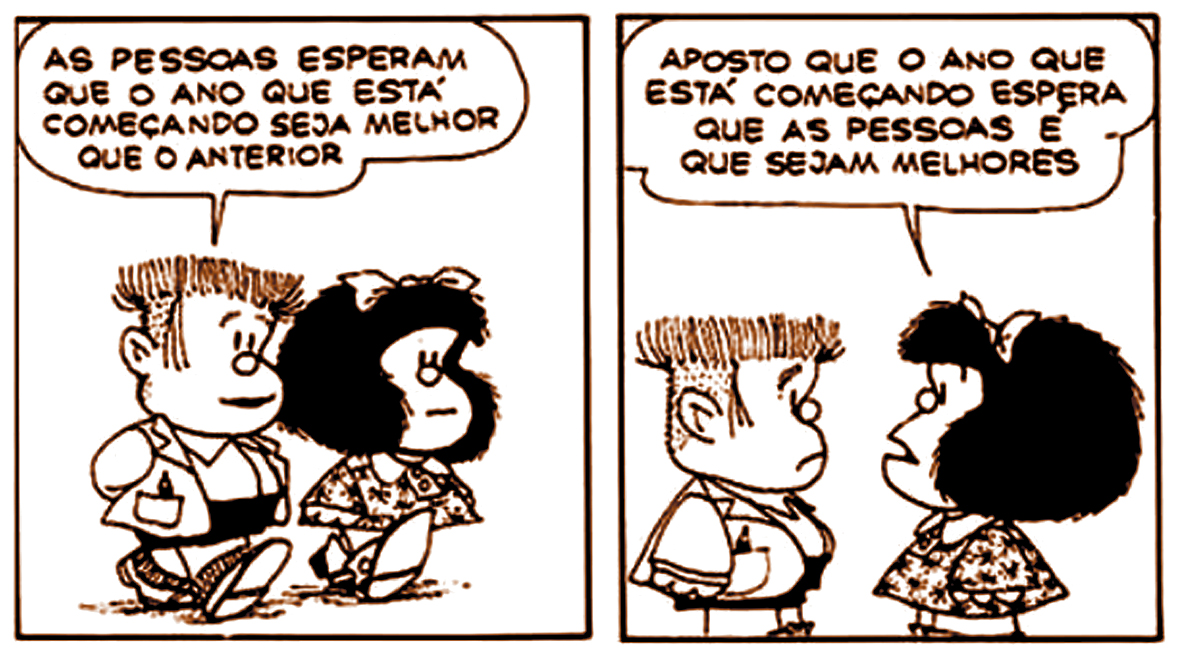
\includegraphics[width=0.75\textwidth]{figuras/mafalda}
%    \begin{flushleft}
%    \flushleft{Fonte: 
%    Elaborado pelo autor.}
%    \end{flushleft}
%    \label{fig:mafalda}
%}
%\end{figure}


%Exemplo de uso de tabela no Latex (Tabela~\ref{tab:tabelaModelo}). Ver página %72 do Manual de Normalização de Trabalhos Acadêmicos do IFCE.
%\begin{table}[th]
%    \centering
%    \caption{Legenda da Tabela no Topo.}
%    \label{tab:tabelaModelo}
%    \begin{tabular}{llll}
%    & Nota mínima & Nota máxima & Nota média\\\hline
%    Ciências Humanas (CH)     & 324,8       & 862,1       & 546,5\\
%    Ciências da Natureza (CN) & 330,6       & 876,4       & 482,2\\
%    Linguagens e Códigos (LC) & 306,2       & 814,2       & 507,9\\
%    Matemática (MT)           & 318,5       & 973,6       & 473,5\\ \hline  
%    \end{tabular}
%    \begin{flushleft}
%    \flushleft{Fonte: 
%    Instituto Brasileiro de Geografia e Estatística - IBGE.}
%    \end{flushleft}
%\end{table}
